\subsection{Task Assignment}\label{subsubsec:task-assignment}
Given the set of posets~$\mathcal{P}_{\varphi}$ derived from the previous
section, this section describes how this set can be used to compute
the optimal assignment of these subtasks. More specifically, we consider
the following sub-problems of task assignment:

\begin{problem}\label{problem:}
Given any poset $P=(\Omega,\, \preceq_{\varphi},\, \neq_{\varphi})$
where~$P\in \mathcal{P}_{\varphi}$,
find the optimal assignment of all subtasks in~$\Omega$ to the multi-agent system
$\mathcal{N}$ such that
(i) all partial ordering requirements in $\preceq_{\varphi},\, \neq_{\varphi}$ are
respected; (ii) the maximum completion time of all subtasks is minimized.
\hfill $\blacksquare$
\end{problem}

To begin with, even without the requirements of partial ordering
and collaborative actions, the above problem includes the multi-vehicle routing
problem~\cite{gini2017multi, khamis2015multi},
and the job-shop scheduling problem~\cite{brucker1994branch} as special instances.
Both problems are well-known to be NP-hard.
Thus, the above problem is also NP-hard and most likely no exact solutions with
polynomial complexity exist.
The most common and straightforward solution is to formulate a Mixed Integer
Linear Program (MILP) with $N \cdot L\cdot (L+1)$ Boolean variables, where~$N$ is the number
of agents and $L$ is the number of subtasks.
Each Boolean variable stands for whether the~$\ell_1$ position in the plan of
agent~$n$ takes the $\ell_2$ subtask or does nothing.
There are two major drawbacks of this approach:
(i) the computation complexity and time grow exponentially with the problem size;
(ii) there is no intermediate solution before the optimal solution is generated,
often via a MILP solver, e.g., CPLEX~\cite{lima2010ibm}.
Both drawbacks hinder the usage of this approach in large-scale real-time applications,
where a timely good solution is far more valuable than the optimal solution.
%========================================
\begin{figure}[t!]
\centering
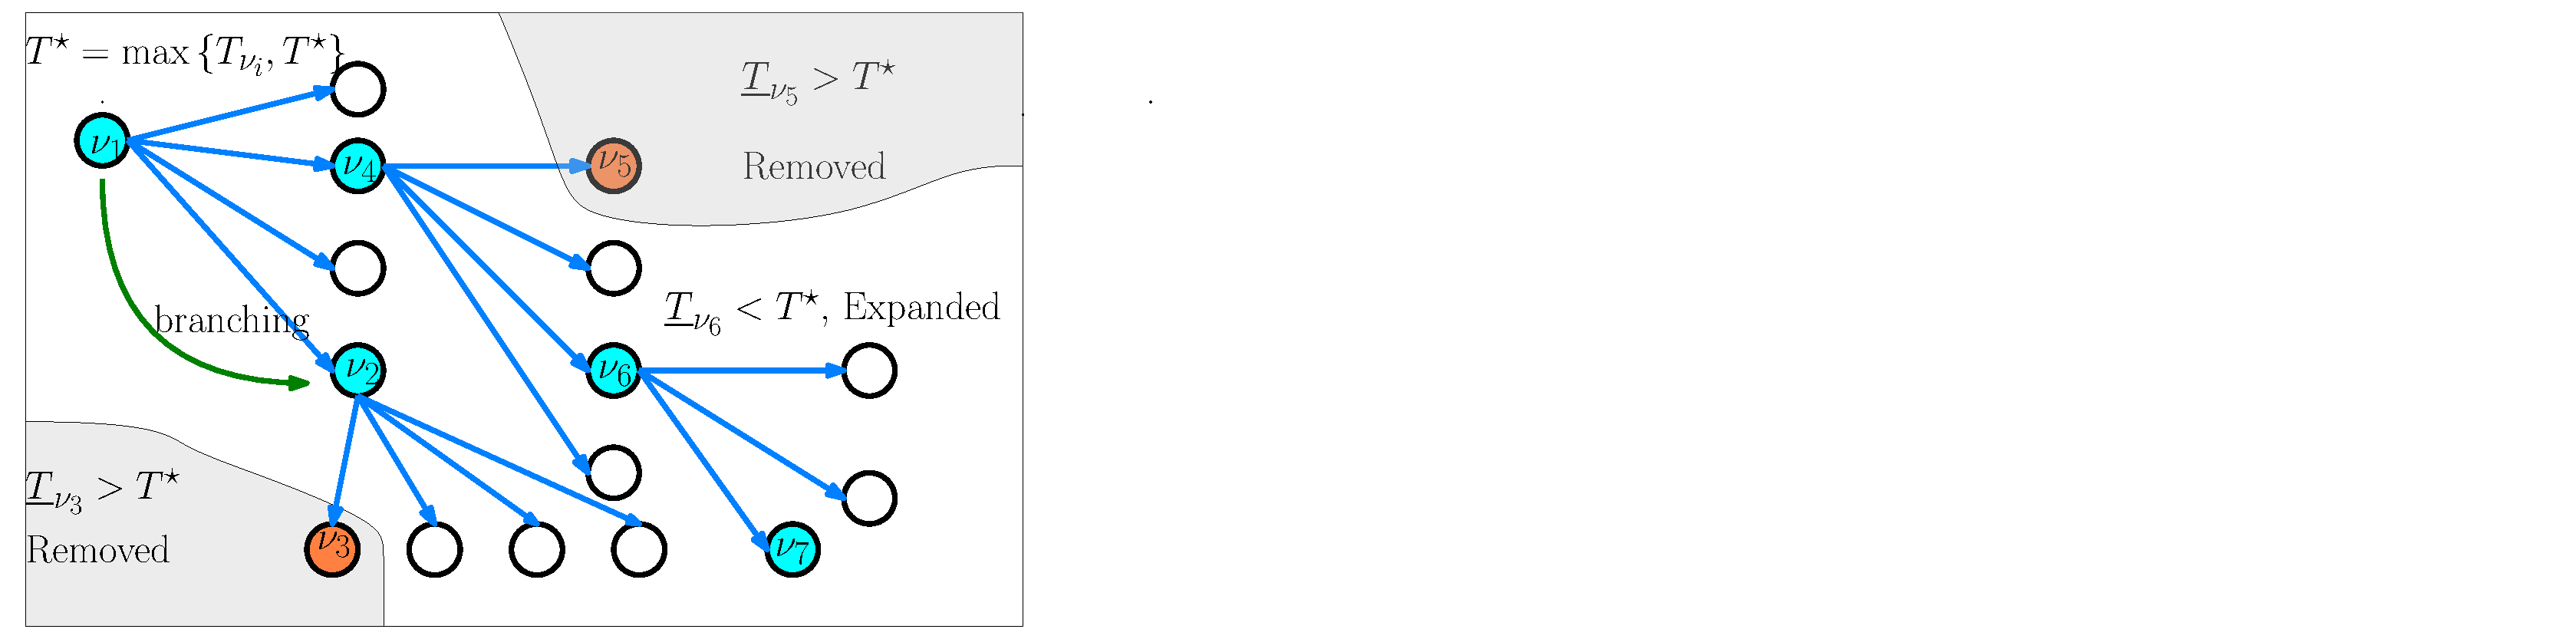
\includegraphics[width=0.9\linewidth]{figures/bnb_graph3.pdf}
%--------------------
\caption{
Illustration of the main components in the BnB search,
i.e., the node expansion and branching to generate explore new nodes (in green arrow);
and the lower and upper bounding to avoid undesired branches (in orange).}
\label{fig:bnb_search_logic}
%--------------------
\end{figure}
%========================================

Motivated by these observations, an anytime assignment
algorithm is proposed in this work based on the Branch and Bound (BnB) search
method~\cite{lawler1966branch, morrison2016branch}.
It is not only complete and optimal, but also anytime, meaning that a good
solution can be inquired within any given time budget.
As shown in Fig.~\ref{fig:bnb_search_logic},
the four typical components of a BnB
algorithm are the node expansion, the branching method,
and the design of the upper and lower bounds.
These components for our application are described in detail below.

\textbf{Node expansion}.
Each node in the search tree stands for one partial assignment of the
subtasks, i.e.,
\begin{equation}\label{eq:node}
\nu = (\tau_1,\,\tau_2,\cdots,\tau_N),
\end{equation}
where $\tau_n$ is the ordered sequence of tasks assigned to agent~$n\in \mathcal{N}$.
To give an example, for a system of three agents,
$\nu=((\omega_1,\omega_2),(),())$ means that two subtasks
$\omega_1,\, \omega_2$ are assigned to agent~$1$,
whereas no tasks to agents~$2$ and $3$.
With slight abuse of notation, denote by
\begin{equation}\label{eq:node-tasks}
\Omega_{\nu}=\{\omega\in\tau_n,\,\forall n\in \mathcal{N}\},
\;\Omega^-_{\nu} = \Omega\backslash \Omega_{\nu},
\end{equation}
where~$\Omega$ is the set of subtasks from $P_\varphi$;
$\Omega_{\nu}$ is the set of subtasks already assigned in node~$\nu$;
and $\Omega^-_{\nu}$ are the remaining unassigned subtasks.
Starting from the root node with zero assignment, the tree is expanded by
generating child nodes where subtasks are partially assigned to the agents,
until all the subtasks are assigned.
More specifically,
let~$\nu$ be the current node of the search tree.
The \emph{next} subtask~$\omega$ to be assigned is chosen from the
poset~$\mathcal{G}_{P_\varphi}$ defined in Def.~\ref{def:poset-graph}
if \emph{all} of its parent subtasks are already assigned, i.e.,
\begin{equation}\label{eq:next-task}
\omega' \in \Omega_\nu, \; \forall \omega' \in \text{Pre}(\omega),
\end{equation}
where~$\Omega_\nu$ is the set of assigned  subtasks from~\eqref{eq:node-tasks};
$\text{Pre}(\omega)$ is the set of preceding or parenting subtasks of $\omega$ in~$\mathcal{G}_{P_\varphi}$.
Once this subtask~$\omega$ is chosen, the succeeding or child node $\nu^+$
of $\nu$ in the search tree is created by assigning $\omega$ to any agent
that is capable of executing $\omega$, i.e.,
\begin{equation}\label{eq:next-agent}
(p_n,\;p_n^+) \in \rightarrow_n,\;\text{and} \; a^+ \in \mathcal{A}^{\texttt{l}}_{n},
\;\text{or}\;a_n^+ \in \mathcal{A}^{\texttt{c}}_{n},
\end{equation}
where~$p_n$ is the current position of agent~$n$ at node~$\nu$,
while~$p^+_n$ is the desired position of agent~$n$ at node~$\nu^+$;
$a^+$ is the desired local action to be performed at node~$\nu^+$,
while $a^+_n$ is the desired collaborative action to be performed
at node $\nu^+$ projected to agent~$n$.
In other words, agent~$n$ can transit to $p^+_n$ and perform $a^+$ or $a_n^+$.
Thus, given node~$\nu=(\tau_1,\cdots,\tau_N)$,
the child node~$\nu^+=(\tau^+_1,\cdots,\tau^+_N)$ is given by
\begin{equation}\label{eq:next-node}
\tau_n^+ = (\tau_n,\;\omega),\;\text{and}\;
\tau_{n'}^+=\tau_{n'},\; \forall n'\neq n.
\end{equation}
If there are multiple agents satisfying the condition in~\eqref{eq:next-agent},
then multiple child nodes are expanded, one for each agent.

\textbf{Branching}.
Given the set of nodes to be expanded,
the branching method determines the order in which these child nodes are
visited.
Many search methods such as breadth first search (BFS), depth first search (DFS)
or $A^\star$ search can be used.
We propose to use $A^\star$ search here as the heuristic function matches well
with the lower bounds introduced in the sequel.
More specifically, the set of child nodes is expanded in the order of
estimated completion time of the whole plan given its current assignment.

%==============================
\begin{algorithm}[t]
\caption{$\texttt{upper\_bound}(\cdot)$: Compute the upper bound of solutions
rooted from a node}
\label{alg:upper_bound}
\SetKwInOut{Input}{Input}\SetKwInOut{Output}{Output}
\Input {Poset~$P_{\varphi}$, node~$\nu$.}
\Output {Assignment~$\overline{J}_\nu$, upper bound~$\overline{T}_\nu$.}
\While(\tcp*[f]{\eqref{eq:node-tasks}}){$\Omega^-_\nu \neq \emptyset$}{
\ForAll{$\omega\in \Omega^-_\nu$\, \text{and}\, $n\in\mathcal{N}$
\label{algline:all-next}}
{Assign $\omega$ to agent~$n$;\\
Compute and save child node~$\nu_{n,\omega}^+$\tcp*{\eqref{eq:next-node}}}
Select~$\nu^{+}_{\star}=\textbf{argmax}_{\nu\in \{\nu_{n,\omega}^+\}}\,\{\eta_{\nu}\}$
\label{algline:compute-eta}\tcp*{\eqref{eq:node-makespan}}
$\nu \leftarrow \nu^{+}_{\star}$; \label{algline:expand-node}\\
}
Compute assignment~$J_\nu$ and makespan~$T_\nu$
\label{algline:return}\tcp*{\eqref{eq:complete-assignment}}
\textbf{Return} $\overline{J}_\nu=J_\nu,\, \overline{T}_\nu=T_\nu$;\\
\end{algorithm}
%==============================

\textbf{Lower and upper bounding}.
For each new node in the search tree, it is checked against the estimated lower
and upper bounds of the optimal solution.
If this node can not produce a better solution, it is discarded from the search
tree and no new nodes will be expanded from it.
Therefore, the accuracy of these bounds effects greatly the
efficiency of a BnB algorithm, which can degenerate to an exhaustive search,
if no such bounds are available.
More specifically, given a node~$\nu$,
the upper bound of all solutions rooted from this node
is estimated via a greedy task assignment policy,
as summarized in Alg.~\ref{alg:upper_bound}:
\begin{equation}\label{eq:upper-bound}
\overline{J}_\nu,\, \overline{T}_\nu  = \texttt{upper\_bound}(\nu,\, P_{\varphi}),
\end{equation}
where~$\overline{T}_\nu$ is upper bound, and~$\overline{J}_\nu$ is the
associated complete assignment \emph{with time stamps}, i.e.,
\begin{equation}\label{eq:complete-assignment}
J = (J_1,\,J_2,\cdots,J_N),
\end{equation}
where~$J_n=((t_1,\,\omega_1),(t_2,\,\omega_2),\cdots,(t_{K_n},\omega_{K_n}))$
is the assignment for agent~$n\in\mathcal{N}$,
and $t_k$ is the starting time for subtask~$\omega_k$,
$\forall (t_k,\,\omega_k)\in J_n$.
From node~$\nu$, any task~$\omega\in \Omega^-_\nu$ is assigned
to any allowed agent~$n\in\mathcal{N}$ in Line~\ref{algline:all-next},
thus generating a set of child nodes~$\{\nu^+_{n,\omega}\}$.
Then, for each node~$\nu\in \{\nu^+_{n,\omega}\}$,
its \emph{concurrency} level~$\eta_{\nu}$ is estimated as follows:
\begin{equation}\label{eq:node-makespan}
T_\nu = \max_{n\in\mathcal{N}} \{T_{\tau_n}\},\;
T^{\texttt{s}}_\nu = \sum_{\omega\in\Omega_\nu}\, T_{\omega}N_\omega,\;
\eta_\nu = \frac{T^{\texttt{s}}_\nu}{T_\nu},
\end{equation}
where node~$\nu=(\tau_1,\cdots,\tau_N)$;~$T_{\tau_n}$ is the execution
time of all subtasks in~$\tau_n$ by agent~$n$;
$T_\nu$ is the current makespan calculate by \eqref{eq:node-makespan};
and $T^{\texttt{s}}_\nu$ is the total execution time of all subtasks~$\omega$
given its duration~$T_\omega$ and the number of participants~$N_\omega$.
Thus, the child node with the highest~$\eta_{\nu}$ is chosen as
the next node to expand in Line~\ref{algline:compute-eta}-\ref{algline:expand-node}.
This procedure is repeated until no subtasks remain unassigned.
Afterwards, a complete assignment~$J_\nu$ with time stamps is obtained by
solving a simple linear program given the sequence of subtasks the last node~$\nu$.
Afterwards, the upper bound~$T_\nu$ is given the makespan of the
complete assignment, as in Line~\ref{algline:return}.

Furthermore, the lower bound of the makespan of all solutions rooted from this
node is estimated via two separate relaxations of the original problem:
one is to consider only the partial ordering constraints while ignoring
the agent capacities;
another is vice versa.
More specifically, let the current node be~$\nu$,
the set of unfinished subtasks is given by~$\Omega^-_\nu$ in~\eqref{eq:node-tasks}.
The first lower bound~$\underline{T}_{\nu,1}$ on the makespan
to accomplish~$\Omega^-_\nu$ is computed via analyzing the poset
graph~$\mathcal{G}_{P_\varphi}=(\Omega,\, E,\, R)$ in~\eqref{def:poset-graph}.
In particularly, consider the directed
graph~$\mathcal{G}'_{P_\varphi}=(\Omega'_\nu,\, E\cap R )$,
where~$\Omega'_\nu$ is the set of nodes associated with the unfinished subtasks,
and the set of edges contains the edge $(\omega',\,\omega)$ that belongs to
both~$\preceq_{\varphi}$ and~$\neq_{\varphi}$.
Then, starting from the set of root nodes that does not have parent nodes,
a BFS procedure is used to traverse all nodes in the graph~$\mathcal{G}'_{P_\varphi}$.
Denote by~$\Gamma^-_{\nu}=\{\tau_{\omega_f,\omega_g}\}$ the set of paths
from any root node~$\omega_f$ to any other node~$\omega_g$ in the graph.
Then, the first lower bound~$\underline{T}_{\nu,1}$ on the makespan is given by
\begin{equation}\label{eq:lower-bound-1}
\underline{T}_{\nu,1} (\nu,\,P_{\varphi})=\textbf{max}_{\tau\in \Gamma^-_\nu} \, \{T_{\tau}\},
\end{equation}
where~$T_{\tau}$ is the accumulated duration
of path~$\tau=\omega_0\omega_1\cdots \omega_P$, i.e., $T_\tau=\sum_{p=1}^PT_{\omega_p}$.
In other words, the lower bound~$\underline{T}_{\nu,1}$ assumes that
there are as many agents as needed for the sub-tasks, while the partial ordering
constraints for the subtasks are ensured.
Secondly, another lower-bound~$\underline{T}_{\nu,2}$ is estimated by
ignoring the partial ordering constraints:
\begin{equation}\label{eq:lower-bound-2}
\underline{T}_{\nu,2} (\nu,\,P_{\varphi})=\frac{\sum_{\omega\in \Omega^-_{\nu}}
T_{\omega} N_{\omega}}{N},
\end{equation}
where~$T_{\omega}$ and~$N_{\omega}$ are the duration and number of agents required
for subtask~$\omega\in \Omega^-_\nu$ as defined in~\eqref{eq:node-makespan}.
%==============================
\begin{algorithm}[t]
\caption{$\texttt{BnB}(\cdot)$: Anytime BnB algorithm for task assignment}
\label{alg:BnB}
\SetKwInOut{Input}{Input}\SetKwInOut{Output}{Output}
\Input {Agents $\mathcal{N}$, poset $P_{\varphi}$, time budget $t_0$.}
\Output {Best assignment $J^\star$ and makespan $T^\star$.}
Initialize root node~$\nu_0$ and queue $Q=\{\nu_0\}$; \label{algline:init-start}\\
Set $T^\star=\infty$ and $J^\star=()$;\label{algline:init-end}\\
\While{($Q$ not empty) or ($time<t_0$)}{
Take node $\nu$ off $Q$;\\
$\overline{J}_\nu,\, \overline{T}_\nu  = \texttt{upper\_bound}(\nu,\, P_{\varphi})$
\tcp*{Alg.~\ref{alg:upper_bound}} \label{algline:upper}
$\underline{T}_\nu = \texttt{lower\_bound}(\nu,\,P_{\varphi})$
\tcp*{\eqref{eq:lower-bound}} \label{algline:lower}
Compute bounds $\overline{T}_\nu$ and $\underline{T}_\nu$
by~\eqref{eq:upper-bound} and~\eqref{eq:lower-bound};\\
\If{$T^\star > \overline{T}_\nu$}{
Set $T^\star=\overline{T}_\nu$ and $J^\star=\overline{J}_\nu$;}
\eIf{$\underline{T}_\nu \geq T^\star$}{
\textbf{Continue} \tcp*{discard branch} \label{algline:discard}}
{Branch on $\nu$ by~\eqref{eq:next-agent} and~\eqref{eq:next-node};\\
Choose new node $\nu^+$ by estimated $\underline{T}_{\nu^+}$; \label{algline:expand}\\
Store $\nu^+$ to $Q$;}
}
\textbf{Return} $J^\star, T^\star$;
\end{algorithm}
%==============================

Consequently, the lower bound on the makespan of all solutions rooted from~$\nu$
is given as the minimum of these two lower bounds above:
\begin{equation}\label{eq:lower-bound}
\underline{T}_\nu = \texttt{lower\_bound}(\nu,\,P_{\varphi})
= \min\,\{\underline{T}_{\nu,1},\, \underline{T}_{\nu,2}\},
\end{equation}
which can be computed efficiently.
It is worth noting that the task assignments associated with~$\underline{T}_\nu$
above is infeasible as it either violates the partial ordering constraints or
the current agent capacities.


%==============================

%------------------------------
\begin{remark}\label{remark:none-milp}
The computation of both the upper and lower bounds are designed
to be free from any integer optimization.
This is intentional to avoid unpredictable solution time caused by
external solvers.
\hfill $\blacksquare$
\end{remark}
%------------------------------

Given the above components, the complete BnB algorithm can be stated as
in Alg.~\ref{alg:BnB}.
In the initialization step in
Line~\ref{algline:init-start}-\ref{algline:init-end},
the root node~$\nu_0$ is created as an empty assignment,
the estimated optimal cost~$T^{\star}$ is set to infinity,
and the queue to store un-visited nodes $Q$ contains only $\nu_0$.
Then, within the time budget, a node $\nu$ is taken from $Q$ for expansion.
The upper and lower bound associated with $\nu$ is computed in
Lines~\ref{algline:upper} and~$\ref{algline:lower}$.
If the upper bound $\overline{T}_{\nu}$ is less than the current best-known
value~$T^{\star}$, then $T^{\star}$ is replaced by $\overline{T}_{\nu}$ and the
associated plan $J^\star$ is saved.
On the other hand, if the lower bound $\underline{T}_{\nu}$ is larger than
the current~$T^\star$, it means no partial solution rooted from this node
can produced a better solution, thus discarded for expansion
in Line~\ref{algline:discard}.
Otherwise, the child node $\nu^+$ of $\nu$ is generated and expanded
according to their estimated lower bounds in Line~\ref{algline:expand}.
This process repeat itself until time elapsed or the whole search tree is
exhausted.

%==============================
\begin{lemma}\label{lemma:BnB-satisfying}
Any task assignment~$J^\star$ obtained from Alg.~\ref{alg:BnB} satisfies
the partial ordering constraints in~$P_{\varphi}$.
\end{lemma}
\begin{proof}
Since the assignment~$J^\star$ belongs to the set of solutions obtained from
the upper bound estimation in Alg.~\ref{alg:upper_bound}
at certain node in the search tree, it suffices to show that any solution
of Alg.~\ref{alg:upper_bound} satisfies the partial ordering constraints.
Regardless of the current node~$\nu$, the set of remaining subtasks
in~$\Omega^-_\nu$ is assigned strictly following the preceding order
in the poset graph as defined in~\eqref{eq:next-task}.
In other words, for any pair~$(\omega_1,\,\omega_2)\in \preceq_{\varphi}\cap \neq_{\varphi}$,
if $\omega_1\in \Omega_\nu$ and $\omega_2\in \Omega^-_\nu$,
then the starting time of~$\omega_2$ is larger than the finishing time of~$\omega_1$.
Similar arguments hold for~$\preceq_{\varphi}$ and~$\neq_{\varphi}$ separately.
\end{proof}
